\documentclass{article}
\usepackage[utf8]{inputenc}

%packages
\usepackage[english]{babel} %Forces American English hyphenation patters
\usepackage{inputenc} % Unicode
\usepackage[margin=0.75in]{geometry}
\usepackage{amsmath, amssymb, amsthm, amsfonts} %AMS Math Packages
\usepackage{textcomp, siunitx, gensymb, wasysym} %Symbol Packages, Textcomp removes certain errors
\usepackage{multicol, fancyhdr} %Page Layout Packages 
\usepackage{graphicx, wrapfig, subcaption} %Figure Packages
\usepackage{xcolor, hyperref, setspace}

\newcommand{\Pb}{\textnormal{Prob}}
\renewcommand{\labelitemii}{$\circ$}


\begin{document}

\begin{spacing}{1.2}
    \begin{center}
        {\Large{Modeling Project III}}
    
        Chris Booth, Michael Dymek, Robin Gates
    
        November 20\textsuperscript{th} 2020
    \end{center}
\end{spacing}

\hrule
\vspace{5pt}
\hrule
\vspace{15pt}
\noindent{\large{\textbf{Net Ecosystem Exchange}}}

\vspace{10pt}

During the day, coastal wetlands act as a net sink of carbon dioxide.  Researchers from West Virginia University were able to measure the net ecosystem exchange (NEE) of several salt marshes in the Waquoit Bay in Massachusetts in 2013 using 4 sites. Their data, along with publicly available data from NOAA has been attached; assume collection was evenly spaced throughout the listed date between 8 am and 4:30 pm. Your task is to develop a model of $NEE$ (measured in $\si{\micro \mole \per \meter^2 \second}$) using:
\begin{itemize}
    \item $PAR$ (photosynthetically active radiation) measured in $\si{\micro \mole \per \meter^2 \second}$
    \item $ST$ (soil temperature) measured in degrees Celsius
    \item $SS$ (pore water salinity) measured in parts per thousand
    \item $PA$ (atmospheric pressure) measured in millibars
    \item $cp$ (specific heat of wet soil) set to $\si{\kilo \joule \per \kilo \gram \per \kelvin}$
    \item $t$ (time) measured in seconds
\end{itemize}

Your model should not be statistically or probabilistically derived; statistical tools can only be used to compute parameters in the model afterwards. You should then use the attached data to discuss the quality of this model. Your report should include the derivation of your model with appropriate justification; the predictions of your model using the data given; and a discussion of the strengths/weaknesses of the model.

\vspace{15pt}
\hrule
\vspace{5pt}
\hrule
\vspace{15pt}

\section{Introduction}We have started to learn that coastal wetlands can act as a sink for the greenhouse gas carbon dioxide. Given the possible global impacts of global warming, which is primarily accelerated by an excess of carbon dioxide in the atmosphere, it is incredibly important that we understand a myriad of ways to help capture it in the earth. The task at hand is to formulate a model of $NEE$ using the parameters listed in the preamble. To do this we use the Buckingham-$\pi$ Theorem and appropriate dimensional analysis to create an model for calculating $NEE$ based on the knowledge of other variables. We'll then use statistical models to determine the best model out of our possible options.


\section{Assumptions} 
A few assumptions had to be made about the provided data in order to be able to model the net ecosystem exchange while keeping as much of the real world complexity as possible.

\begin{enumerate}
\vspace{-2.5mm}
    \item All parameters that affect $NEE$ are given in the data set.
    \begin{itemize}
    \vspace{-2.5mm}
    \item \textit{Reasoning:} Adding additional parameters would require extensive research and understanding of how wetlands absorb CO$_2$. Outside of the given data set, any additional parameters could affect the model drastically.
    \end{itemize}
    \vspace{-2.5mm}
    
    \item The dimensionless function is a standard basic function such as linear or quadratic.
    \begin{itemize}
    \vspace{-2.5mm}
    \item \textit{Reasoning:} We assume this function will take the form of something basic in order to be able to perform a regressional analysis on the data. This assumption will help to avoid any unnecessary complexity in the final model derivation.
    \end{itemize}
    \vspace{-2.5mm}
    
\end{enumerate}

\section{Formulating a Model}

We wish to find a modeling function $f$ such that $NEE = f(PAR,ST,SS,Pa,cp,t)$ supposing that one exists. To do so, it is helpful to use dimensional analysis. First, to establish a set a fundamental units, let $L_1 = \si{\micro \mole}$, $L_2 = \si{\meter}$, $L_3 = \si{\second}$, $L_4 = \si{\celsius}$, and $L_5 = \si{\kilo \gram}$.\medskip

Normally $SS$, porewater salinity, is measured in parts per thousand, which is a dimensionless quantity. However, since we know the density of water, the units of $SS$ can be written as $\si{\kilogram \per \meter^3}$, where we substitute the mass of water as the density of water multiplied by the mass of water which cancels with the mass of salt.\medskip

We still need to do a little more massaging before we are ready to proceed. Soil temperature ($ST$) is measured in degrees centigrade, while the specific heat of wet soil ($cp$) is measured in degrees Kelvin. However, because specific heat is the energy necessary to change the temperature of a substance by one degree and a change of one degree Kelvin is the same as a change by one degree centigrade, we can instead consider $cp$ to be measured with degrees centigrade. \medskip

Thus, we have the dimensions of our quantities of interest can be expressed as

\begin{align*}
    [NEE] &= L_1L_2^{-2}L_3^{-1}\\
    [PAR] &= L_1L_2^{-2}L_3^{-1}\\
    [ST]  &= L_4\\
    [SS]  &= L_2^{-3}L_5\\
    [PA]  &= L_2^{-1}L_3^{-3}L_5\\
    [cp]  &= L_2^2L_3^{-2}L_4^{-1}\\
    [t]  &= L_3
\end{align*}

First, we can note that $[NEE/PAR] = 1$. Thus $NEE/PAR = \Pi = (PAR)^{-1}f(PAR,ST,SS,Pa,cp,t)$ is a function with dimensionless output. If we arbitrarily let our primary quantities be $PAR,ST,SS,Pa,t$, we have that the dimensions of $cp$ can be expressed in terms of these quantities: $[cp] = L_2^2L_3^{-2}L_4^{-1} = [(ST)^{-1}(SS)^{-1}(PA)^{1}]$. Thus, the quantity $\Pi_1 = (cp)(ST)(SS)(PA)^{-1}$ is dimensionless and $cp = \Pi_1(ST)^{-1}(SS)^{-1}(PA)^{1}$.\medskip

Subsequently, we have that 
$$\Pi = PAR^{-1} f(PAR, ST,SS, Pa,cp,t) =  PAR^{-1}f(PAR,ST,SS,Pa,\Pi_1(ST)^{-1}(SS)^{-1}(PA)^{1},t).$$

Defining $F(x_1,x_2,x_3,x_4,x_5,x_6) = (x_1)^{-1}f(x_1,x_2,x_3,x_4, x_2^{-1}x_3^{-1}x_4^{-1}x_5,x_6)$, we have $\Pi = F(PAR, ST, SS, Pa, \Pi_1, t)$. Note that, $\Pi$ is dimensionless and is thus invariant under scaling of dimensions. If the function $F$ had any dependence on the primary quantities, it's output would be affected by a scaling of the dimensions of that quantity. Thus, $F$ is independent of our primary quantities and we can re-express $NEE/PAR = \Pi = F(\Pi_1)$. Subsequently, $$NEE = (PAR) F((cp)(ST)(SS)(PA)^{-1}).$$\medskip

In the next section, we postulate several potential functions $F$ and evaluate the accuracy of the models implied by those choices.\\

\section{Estimate Parameters and Test the Model}
Using the Buckingham-$\pi$ theorem, we concluded that
$$NEE \propto \left(PAR\right)f\left( \frac{\left(cp\right)\left( ST\right) \left(SS\right)}{PA} \right).$$
Now, if we want to move further with this model, we will need to use some data analysis to determine the best fitting function and the constant of proportionality. \medskip

To determine the best fitting function, we will run linear regressions for different choices of $f$. Once we have found the function choice that best fits our data, the slope of our regression line will be the constant of proportionality. \medskip

Researchers from West Virginia University were able to measure the net ecosystem exchange of several salt marshes in the Waquoit Bay in Massachusetts in 2013 using 4 sites.  Their data, along with publicly available data from NOAA will comprise our data. Our data analysis will consist of taking our dataset, and running a linear regression on the following functions:
\begin{align*}
    NEE &= \left(PAR\right)\left(\frac{(cp)(SS)(ST)}{PA}\right) \\
    NEE &= \left(PAR\right)\left(\frac{(cp)(SS)(ST)}{PA}\right)^2 \\
    NEE &= \left(PAR\right)\left(\frac{(cp)(SS)(ST)}{PA}\right)^{1/2} \\
    NEE &= \left(PAR\right)\ln\left(\frac{(cp)(SS)(ST)}{PA}\right)
\end{align*}

For each function, we evaluated both the left and righthand sides of each equation. After plotting them, we ran a linear regression on each model to determine the best fit line. We then used the residuals and the $r^2$ value to determine which model best fit the data given. Finally, we'll take the slope parameter from the best fit line and set it equal to the proportionality constant. To aid in the checking of our work, we encourage readers to check the dataset using the R code attached with this paper. \medskip

In the appendix section, we've attached the scatter plots with best fit lines, regression fit data, along with the diagnostic plots used to help evaluate goodness of fit. From those, we can see that the linear and quadratic fits both have the largest $r^2$ value, which suggests that they both fit the data the best. From there, we can look at the residuals vs. fitted graph of each to see that the quadratic is a more consistent fit, so we will chose that model as the best fit. The other two tested models have both smaller $r^2$ values, and worse looking residual graphs. All of this put together, we find that
$$NEE = \left(-5.853\times 10^{-9}\right)\left( PAR \right) \left(\frac{(cp)(SS)(ST)}{PA}\right)^2.$$

\section{Conclusions and Discussion}
With our assumptions given, we were able to use dimensional analysis to create a model for predicting NEE of $CO_2$ for coastal wetlands. In particular, we used the data gathered from several sites in the Waquoit Bay in Massachusetts. Since the data came from a cluster of sites that are relatively close together, there may be other factors involved in predicting NEE that weren't observed in the data. This ties in to the first assumption that we made in that we had all the necessary elements to predict the NEE. So while our final model might work for the sites in Waquoit Bay, this version may not accurately represent other wetland regions.\\

Additionally, with our second assumption we settled on the quadratic function as it had a larger $R^2$ value than the other models, and seemed to have a better residual graph. Other areas might have different representations in the data which could alter the regression models we ran. This could ultimately lead to different functions providing better fits than what we limited ourselves in choosing. Even though we chose the quadratic function because it had a decent $R^2$ value, it wasn't high enough to consider the model to be a good fit for predicting NEE. This could possibly suggest that there are other variables that were not included in the data that would be needed to create a better fit.\\ 

In discussing shortcomings to the model, we did not encounter too many. Dimensional analysis was a useful tool in creating the final model. This approach however, felt as though we were creating a model in order to fit the data given. Specifically we were picking a nice enough function (linear vs. quadratic) that would best fit the provided data. Lastly, an additional aspect of analysis that could have proved useful would have been to examine how changing one quantity with the others fixed constant would have altered the model and results. Due to time constraints however this analysis was omitted.

\section*{Contributions}

\begin{itemize}
\item \textbf{Chris:} Helped with all discussions, wrote assumptions and conclusions section,  helped outline final writeup.  

\item \textbf{Michael:} Ran all the regressional analysis, and wrote corresponding section. Helped in discussions and formulating the model.

\item \textbf{Robin:} Used dimensional analysis to help formulate the model and wrote the corresponding section.

\end{itemize}
\newpage

\section{Appendix: R Code}
\begin{verbatim}
    ####First, I need to set my working directory and import the data from the csv.####
  #The file path and the file name will need to be changed to suit the data file you're using
  setwd("C:/Users/happy/Library of Michael/Western/Math 510 - Mathematical Modeling/Projects/Project 3")
  dataset = read.csv("Workable Dataset.csv")
  functionInput = 1480*(dataset$ST * dataset$SS)/(dataset$Pr)
  linearFunctionData = dataset$PAR * functionInput
  squareFunctionData = dataset$PAR * functionInput^2
  cubeFunctionData = dataset$PAR * functionInput^3
  fourFunctionData = dataset$PAR * functionInput^4
  rootFunctionData = dataset$PAR * functionInput^(1/2)
  exponentialFunctionData = dataset$PAR * exp(functionInput)
  logarithmFunctionData = dataset$PAR * log(functionInput)
  reciprocalFunctionData = dataset$PAR * (1/functionInput)
  
####Linear Regression####
  linearModel <- lm(dataset$NEE ~ 0 + linearFunctionData)
  summary(linearModel)

  par(mfrow=c(1,1))
  plot(linearFunctionData, dataset$NEE, 
       main="Regression of NEE = PAR * ((cp) (SS) (ST)/ (PA))", 
       sub="Determining if the function is linear",
       xlab="PAR * ((cp) (SS) (ST)/ (PA))", ylab="NEE",
       col.main="red", col.lab="blue", col.sub="black")
  abline(linearModel)

  par(mfrow=c(2,2))
  plot(linearModel, col.main="black", col.lab="blue")
  title(main = "Diagnostic Plots for linear model", line = -1.5, 
        outer = TRUE, col.main="red")
  
####Square Regression####
  squareModel <- lm(dataset$NEE ~ 0 + squareFunctionData)
  summary(squareModel)
  
  par(mfrow=c(1,1))
  plot(squareFunctionData, dataset$NEE, 
       main="Regression of NEE = PAR * ((cp) (SS) (ST)/ (PA))^2", 
       sub="Determining if the function is quadratic",
       xlab="PAR * ((cp) (SS) (ST)/ (PA))^2", ylab="NEE",
       col.main="red", col.lab="blue", col.sub="black")
  abline(squareModel)
  
  par(mfrow=c(2,2))
  plot(squareModel, col.main="black", col.lab="blue")
  title(main = "Diagnostic Plots for quadratic model", line = -1.5, 
        outer = TRUE, col.main="red")
  
####Logarithm Regression####
  logarithmModel <- lm(dataset$NEE ~ 0 + logarithmFunctionData)
  summary(logarithmModel)
  
  par(mfrow=c(1,1))
  plot(logarithmFunctionData, dataset$NEE, 
       main="Regression of NEE = PAR * log((cp) (SS) (ST)/ (PA))", 
       sub="Determining if the function is logarithmic",
       xlab="PAR * ln((cp) (SS) (ST)/ (PA))", ylab="NEE",
       col.main="red", col.lab="blue", col.sub="black")
  abline(logarithmModel)
  
  par(mfrow=c(2,2))
  plot(logarithmModel, col.main="black", col.lab="blue")
  title(main = "Diagnostic Plots for logarithmic model", line = -1.5, 
        outer = TRUE, col.main="red")
  
####Root Regression####
  rootModel <- lm(dataset$NEE ~ 0 + rootFunctionData)
  summary(rootModel)
  
  par(mfrow=c(1,1))
  plot(rootFunctionData, dataset$NEE,
       main="Regression of NEE = PAR * ((cp) (SS) (ST)/ (PA))^(1/2)", 
       sub="Determining if the function is a square root",
       xlab="PAR * ((cp) (SS) (ST)/ (PA))^(1/2)", ylab="NEE",
       col.main="red", col.lab="blue", col.sub="black")
  abline(rootModel)
  
  par(mfrow=c(2,2))
  plot(rootModel, col.main="black", col.lab="blue")
  title(main = "Diagnostic Plots for square root model", line = -1.5, 
        outer = TRUE, col.main="red")
\end{verbatim}
\begin{figure}[p] %Linear Model Figure
    \centering
    \begin{subfigure}{0.49\textwidth}
        \centering
        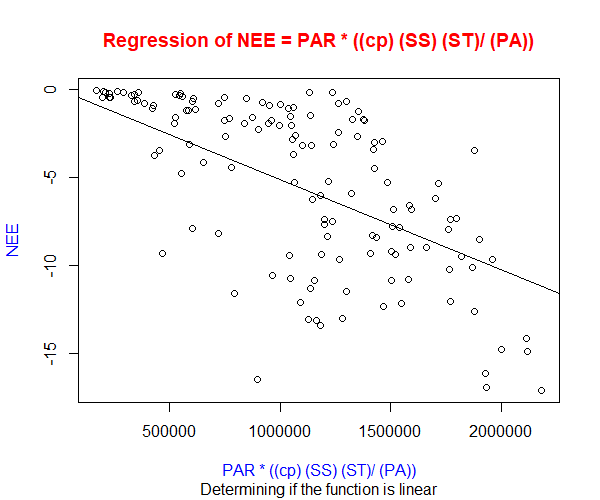
\includegraphics[width = 0.95\textwidth]{Linear_Regression.png}
    \end{subfigure}
    \begin{subfigure}{0.49\textwidth}
        \centering
        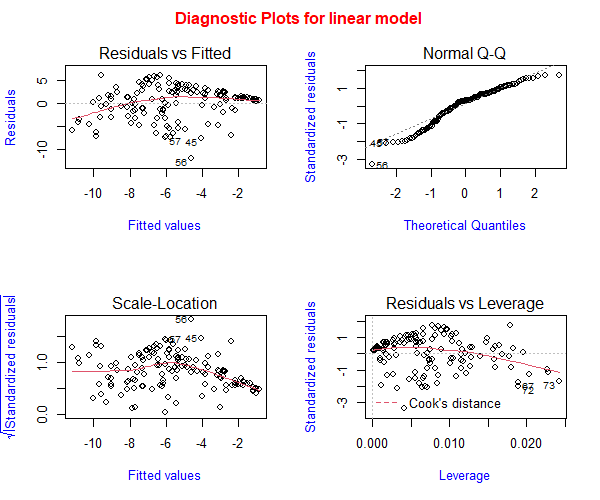
\includegraphics[width = 0.95\textwidth]{Linear_Diagnostics.png}
    \end{subfigure}
    \begin{subfigure}{\textwidth}
        \centering
        \vspace{0.5cm}
        \begin{tabular}{|c|c|}
        \hline
        Parameter & Value \\ \hline \hline
        Slope Estimate & $-5.117e-06$ \\ \hline
        Multiple $r^2$ & 0.7459 \\ \hline
        \end{tabular}
    \end{subfigure}
    \caption{Linear Regression Results}
\end{figure}
\begin{figure}[p] %Quadratic Model Figure
    \centering
    \begin{subfigure}{0.49\textwidth}
        \centering
        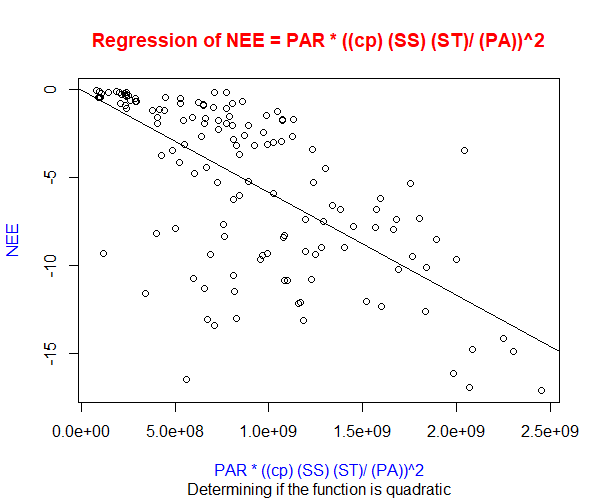
\includegraphics[width = 0.95\textwidth]{Quadratic_Regression.png}
    \end{subfigure}
    \begin{subfigure}{0.49\textwidth}
        \centering
        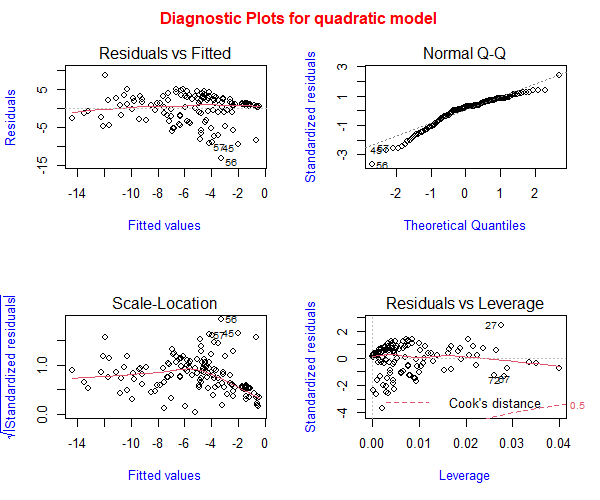
\includegraphics[width = 0.95\textwidth]{Quadratic_Diagnostics.png}
    \end{subfigure}
    \begin{subfigure}{\textwidth}
        \centering
        \vspace{0.5cm}
        \begin{tabular}{|c|c|}
        \hline
        Parameter & Value \\ \hline \hline
        Slope Estimate & $-5.853e-09$ \\ \hline
        Multiple $r^2$ & 0.7459 \\ \hline
        \end{tabular}
    \end{subfigure}
    \caption{Quadratic Regression Results}
\end{figure}
\begin{figure}[p] %Logarithmic Model Figure
    \centering
    \begin{subfigure}{0.49\textwidth}
        \centering
        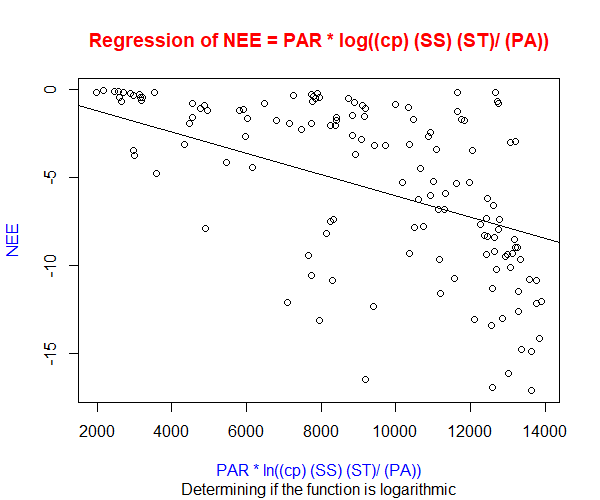
\includegraphics[width = 0.95\textwidth]{Logarithm_Regression.png}
    \end{subfigure}
    \begin{subfigure}{0.49\textwidth}
        \centering
        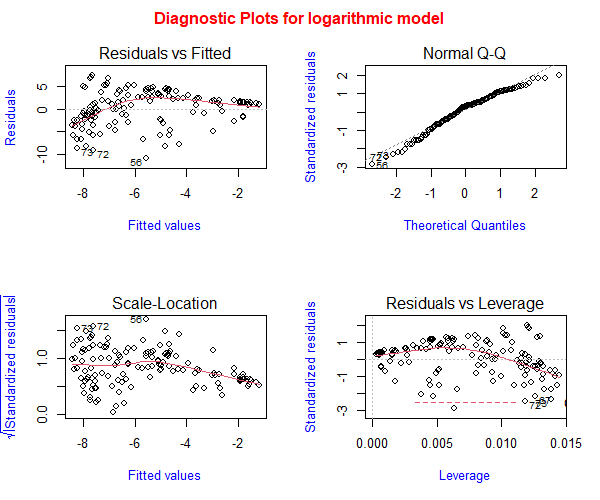
\includegraphics[width = 0.95\textwidth]{Logarithm_Diagnostics.png}
    \end{subfigure}
    \begin{subfigure}{\textwidth}
        \centering
        \vspace{0.5cm}
        \begin{tabular}{|c|c|}
        \hline
        Parameter & Value \\ \hline \hline
        Slope Estimate & $-6.061e-04$ \\ \hline
        Multiple $r^2$ & 0.7113 \\ \hline
        \end{tabular}
    \end{subfigure}
    \caption{Quadratic Regression Results}
\end{figure}
\begin{figure}[p] %Root Model Figure
    \centering
    \begin{subfigure}{0.49\textwidth}
        \centering
        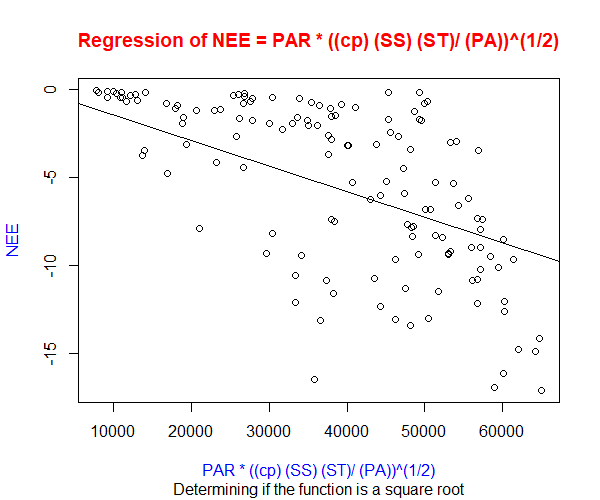
\includegraphics[width = 0.95\textwidth]{Root_Regression.png}
    \end{subfigure}
    \begin{subfigure}{0.49\textwidth}
        \centering
        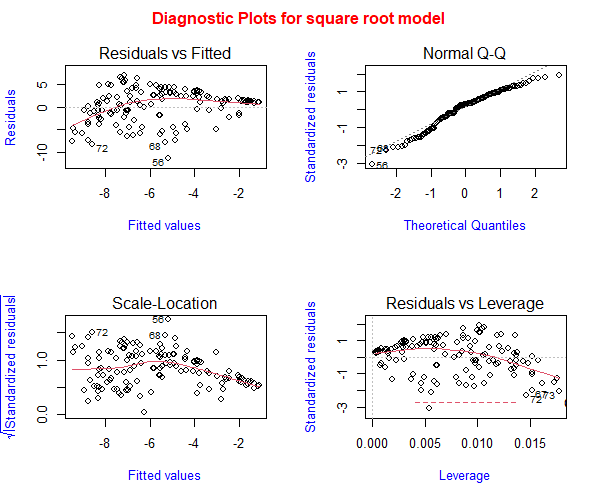
\includegraphics[width = 0.95\textwidth]{Root_Diagnostics.png}
    \end{subfigure}
    \begin{subfigure}{\textwidth}
        \centering
        \vspace{0.5cm}
        \begin{tabular}{|c|c|}
        \hline
        Parameter & Value \\ \hline \hline
        Slope Estimate & $-1.455e-04$ \\ \hline
        Multiple $r^2$ & 0.7303 \\ \hline
        \end{tabular}
    \end{subfigure}
    \caption{Square Root Regression Results}
\end{figure}
\end{document}